\section{Benchmark NIST-2 "Reentrant Corner"}
\label{sec:bench-2}

This is a standard benchmark for adaptive FEM algorithms.
A reentrant corner is nothing more than an internal or inside corner.
It is a very frequent problem and it can cause the error of the solution
calculated by an adaptive method to converge very slowly or not to converge at all.
The exact solution of this problem is smooth but it contains
singular gradient in the reentrant corner.
The equation solved is the Laplace's equation.

\begin{equation} \label{laplace}
-\Delta u = 0,
\end{equation}
in the domain $\Omega = (-1, 1)^2$, with a unit square
section removed from the bottom part of the positive $x$ axis.
Equation (\ref{laplace}) equipped with Dirichlet
boundary conditions given by the exact solution:

\begin{equation}\label{exact-nist-2}
u(x, y) = r^{\alpha}\sin(\alpha \theta),
\end{equation}

where $\alpha = \pi / \omega$, $r = \sqrt{x^2+y^2}$,
and $\theta = tan^{-1}(y/x)$. Here $\omega $ determines
the angle of the reentrant corner.
The solution of NIST-2 with $\omega = 3 \pi / 2$
is shown in Fig. \ref{fig:sln-nist02}.

\begin{figure}[!ht]
\centering
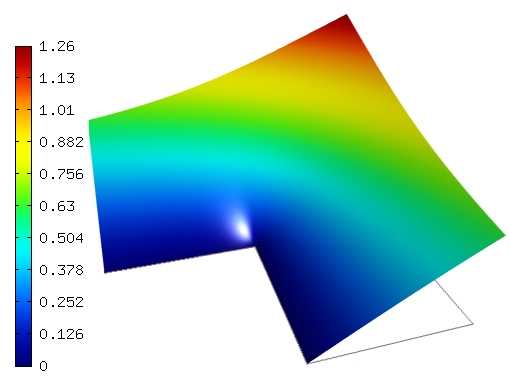
\includegraphics[height=5cm]{nist/nist-2/solution.png}
\caption{The solution to NIST-2 benchmark problem.}
\label{fig:sln-nist02}
\end{figure}
\noindent

The goal of the benchmark is to reach a relative error below
$10^{-1}$~\% in the $H^1$-norm with as few DOFs as possible.
We begin with adaptive $hp$-FEM with possible anisotropic refinements.
The initial mesh is shown in Fig. \ref{fig:nist-2-hp-aniso} (left).
In a few adaptivity steps, the polynomial degree of elements is increased
anisotropically.
The resulting mesh with 622 DOF is shown in Fig. \ref{fig:nist-2-hp-aniso} (right).

\begin{figure}[!ht]
\centering
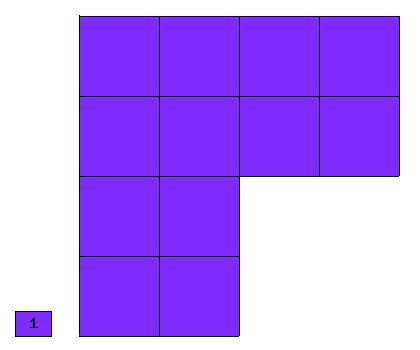
\includegraphics[height=5cm]{nist/nist-2/mesh_hp_aniso_init.png}\ \
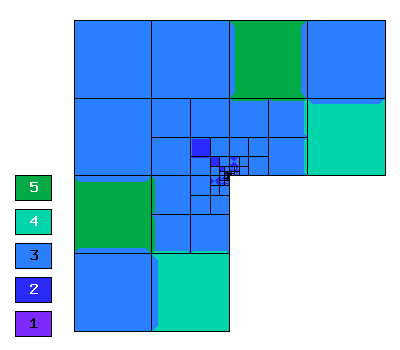
\includegraphics[height=5cm]{nist/nist-2/mesh_hp_aniso.png}
\vspace{-2mm}
\caption{Initial mesh (left) and final mesh (right) for $hp$-FEM with anisotropic refinements.}
\label{fig:nist-2-hp-aniso}
\end{figure}

The final relative error estimate in $H^1$-norm was 8.15289e-02 \%,
and it was identical to the exact error in all printed digits.
We also solved this benchmark with adaptive $h$-FEM
with linear (left) and quadratic (right)
elements, with anisotropic refinements enabled.
Final meshes for the $h$-FEM computations are shown
in Fig. \ref{fig:nist-2-h-aniso}.

\begin{figure}[!ht]
\centering
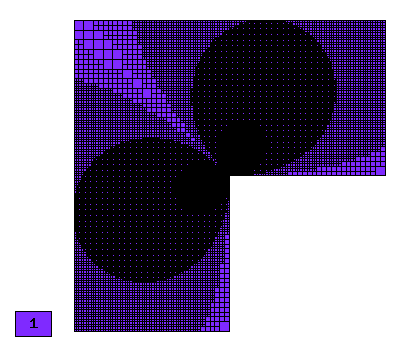
\includegraphics[height=5cm]{nist/nist-2/mesh_h1_aniso.png}\ \
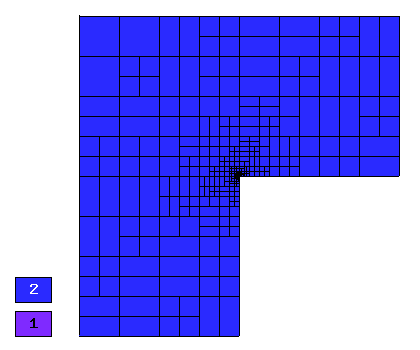
\includegraphics[height=5cm]{nist/nist-2/mesh_h2_aniso.png}
\vspace{-2mm}
\caption{Final mesh for $h$-FEM anisotropic refinements with linear and quadratic elements.}
\label{fig:nist-2-h-aniso}
\end{figure}

Figs. \ref{fig:nist-2-conv} compare all
three approaches to automatic adaptivity from the point
of view of DOF and CPU convergence.

\begin{figure}[!ht]
\centering
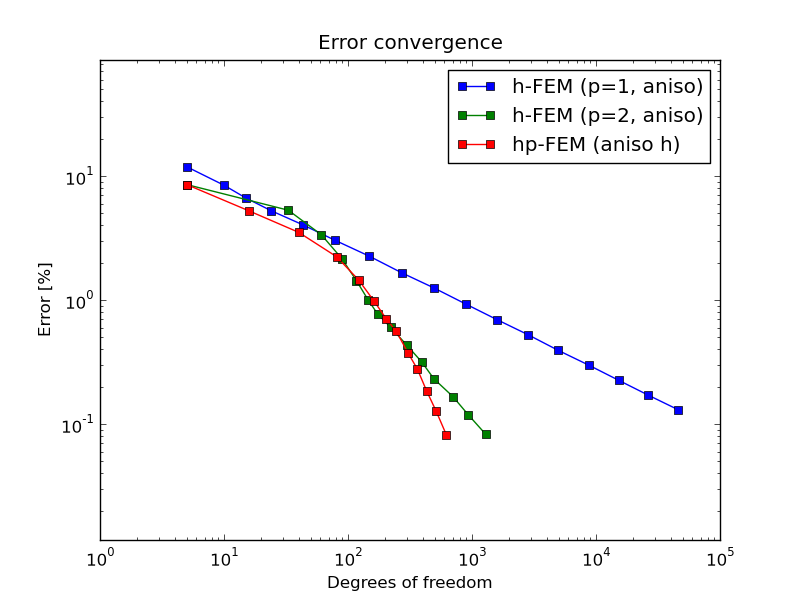
\includegraphics[height=5cm]{nist/nist-2/conv_dof_aniso.png}\ \
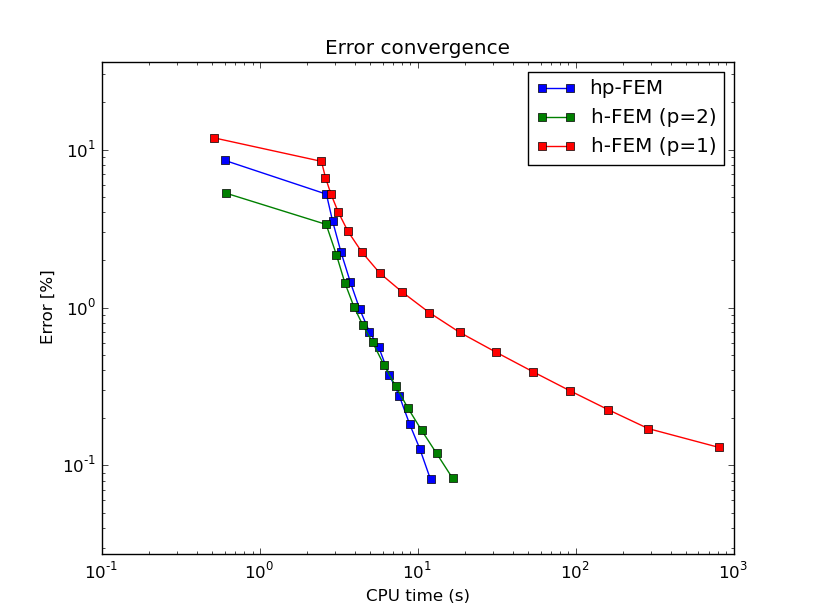
\includegraphics[height=5cm]{nist/nist-2/conv_cpu_aniso.png}
\caption{DOF and CPU time convergence graphs.}
\label{fig:nist-2-conv}
\end{figure}

